% !TEX root = ../main.tex
\section{Kết quả và Phân tích}

Để đánh giá hiệu quả của phương pháp đề xuất, chúng tôi đã tiến hành một chuỗi thực nghiệm trên hệ thống với các bộ tham số di truyền tiêu chuẩn. Quần thể được thiết lập ở quy mô 240 cá thể với tỷ lệ lai ghép 0.95 và tỷ lệ đột biến 0.2. Các thực nghiệm được triển khai trên 5 bộ dữ liệu ngẫu nhiên khác nhau (seeds) để kiểm chứng tính ổn định và khả năng lặp lại của thuật toán. Kết quả thống kê chi tiết từ các lần chạy được tổng hợp trong các bảng dữ liệu dưới đây.

\begin{table}[H]
    \centering
    \begin{tabular}{|l|c|}
    \hline
    \textbf{Chỉ số hiệu suất} & \textbf{Giá trị trung bình} \\ \hline
    Tỷ lệ tìm thấy lịch hợp lệ (Feasible Rate) & 100\% \\ \hline
    Số vi phạm ràng buộc cứng (Hard Violations) & 0.0 \\ \hline
    Phạt mềm trung bình (Avg Soft Penalty) & 10.52 \\ \hline
    Độ lệch chuẩn phạt mềm (Std Soft Penalty) & 3.42 \\ \hline
    Số thế hệ thực thi trung bình (Avg Generations) & 100 \\ \hline
    \end{tabular}
    \caption{Tổng hợp kết quả hiệu suất trung bình trên 5 lần chạy thực nghiệm.}
    \label{tab:summary_results}
\end{table}

Phân tích dữ liệu thực nghiệm cho thấy một sự ổn định đáng kể trong khả năng tìm kiếm nghiệm khả thi của thuật toán. Trong tất cả các lần chạy, hệ thống đều đạt được tỷ lệ lịch học hợp lệ là 100\% mà không vi phạm bất kỳ ràng buộc cứng nào. Chỉ số phạt mềm trung bình đạt mức 10.52 với độ lệch chuẩn 3.42, phản ánh chất lượng lịch học đồng nhất giữa các bộ dữ liệu khác nhau. Đáng chú ý là thuật toán thường hội tụ và kích hoạt cơ chế dừng sớm sau khoảng 100 thế hệ, minh chứng cho tính hiệu quả của chiến lược khởi tạo bằng heuristic trong việc định hướng sớm vùng nghiệm tối ưu.

\begin{table}[H]
    \centering
    \begin{tabular}{|c|c|c|c|c|c|}
        \hline
        \textbf{Seed} & \textbf{Số thế hệ} & \textbf{Độ thích nghi} & \textbf{Tổng phạt} & \textbf{Vi phạm cứng} & \textbf{Phạt mềm} \\ \hline
        40 & 100 & 0.0771 & 11.9708 & 0 & 11.9708 \\ \hline
        41 & 100 & 0.0646 & 14.4788 & 0 & 14.4788 \\ \hline
        42 & 100 & 0.0708 & 13.1329 & 0 & 13.1329 \\ \hline
        43 & 100 & 0.1175 & 7.5132 & 0 & 7.5132 \\ \hline
        44 & 100 & 0.1533 & 5.5213 & 0 & 5.5213 \\ \hline
    \end{tabular}
    \caption{Chi tiết kết quả thực nghiệm theo từng bộ giá trị ngẫu nhiên (seed).}
\end{table}

Về mặt động lực học của quá trình tiến hóa, biểu đồ quá trình thích nghi cho thấy số lượng vi phạm ràng buộc cứng được triệt tiêu hoàn toàn ngay từ những thế hệ đầu tiên nhờ sự kết hợp giữa heuristic seeding và hàm sửa lỗi. Trong khi đó, độ thích nghi trung bình của quần thể liên tục được cải thiện thông qua việc tối ưu hóa các thành phần phạt mềm, cụ thể là việc phân bổ đều các lớp học giữa các khung giờ và phòng học để tránh tình trạng tập trung quá mức vào một thời điểm nhất định.

\begin{figure}[H]
    \centering
    
\includegraphics[width=0.8\textwidth]{images/fitness_plot.png}
    \caption{Biểu đồ diễn biến của độ thích nghi và số lượng vi phạm ràng buộc theo thế hệ.}
    \label{fig:fitness_plot}
\end{figure}

Sự khác biệt về giá trị phạt mềm giữa các seed, dao động từ mức thấp nhất là 5.52 cho đến cao nhất là 14.48, cho thấy cấu trúc dữ liệu đầu vào có ảnh hưởng nhất định đến độ khó của việc tối ưu hóa. Tuy nhiên, việc duy trì được vi phạm cứng bằng không trên mọi trường hợp khẳng định rằng thuật toán đã đạt được mục tiêu cơ bản về tính khả thi của lịch học, đáp ứng đầy đủ các yêu cầu khắt khe về mặt tổ chức đào tạo đã đề ra trong mô hình bài toán.

\begin{figure}[H]
    \centering
    \begin{minipage}{0.48\textwidth}
        \centering
        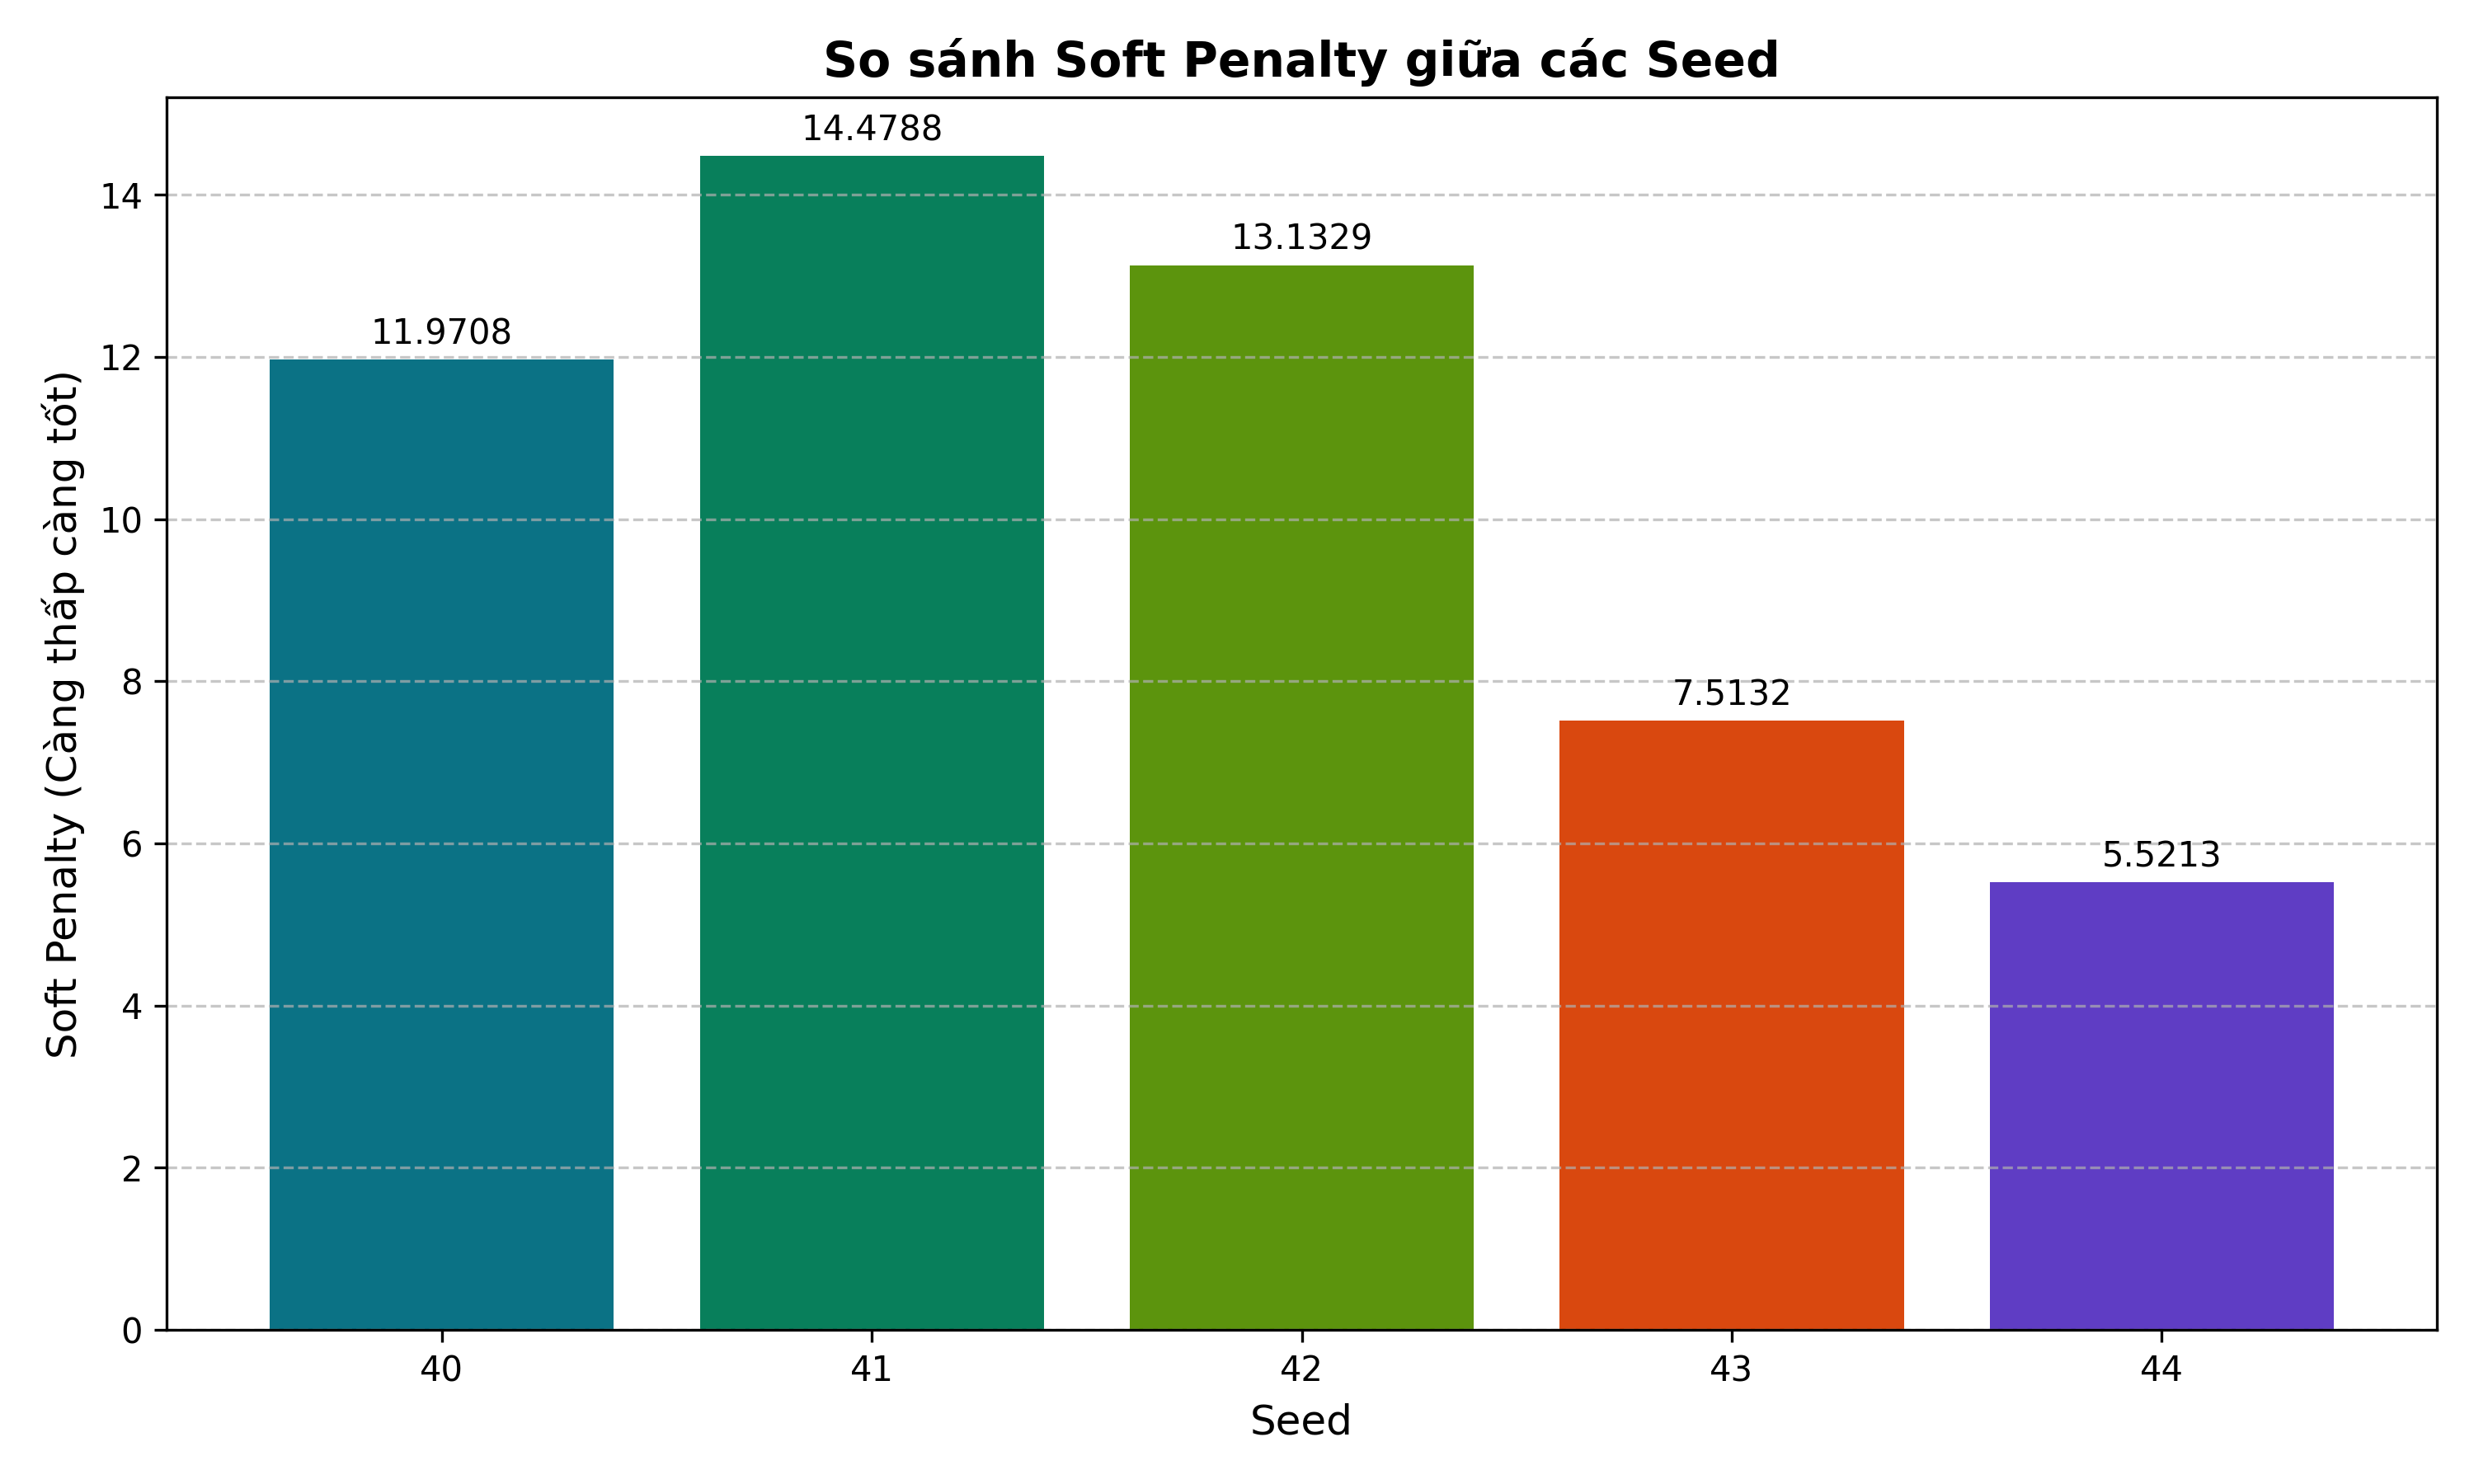
\includegraphics[width=\textwidth]{images/soft_penalty_comparison.png}
        \caption{So sánh chỉ số phạt mềm giữa các seed thực nghiệm.}
    \end{minipage}
    \hfill
    \begin{minipage}{0.48\textwidth}
        \centering
        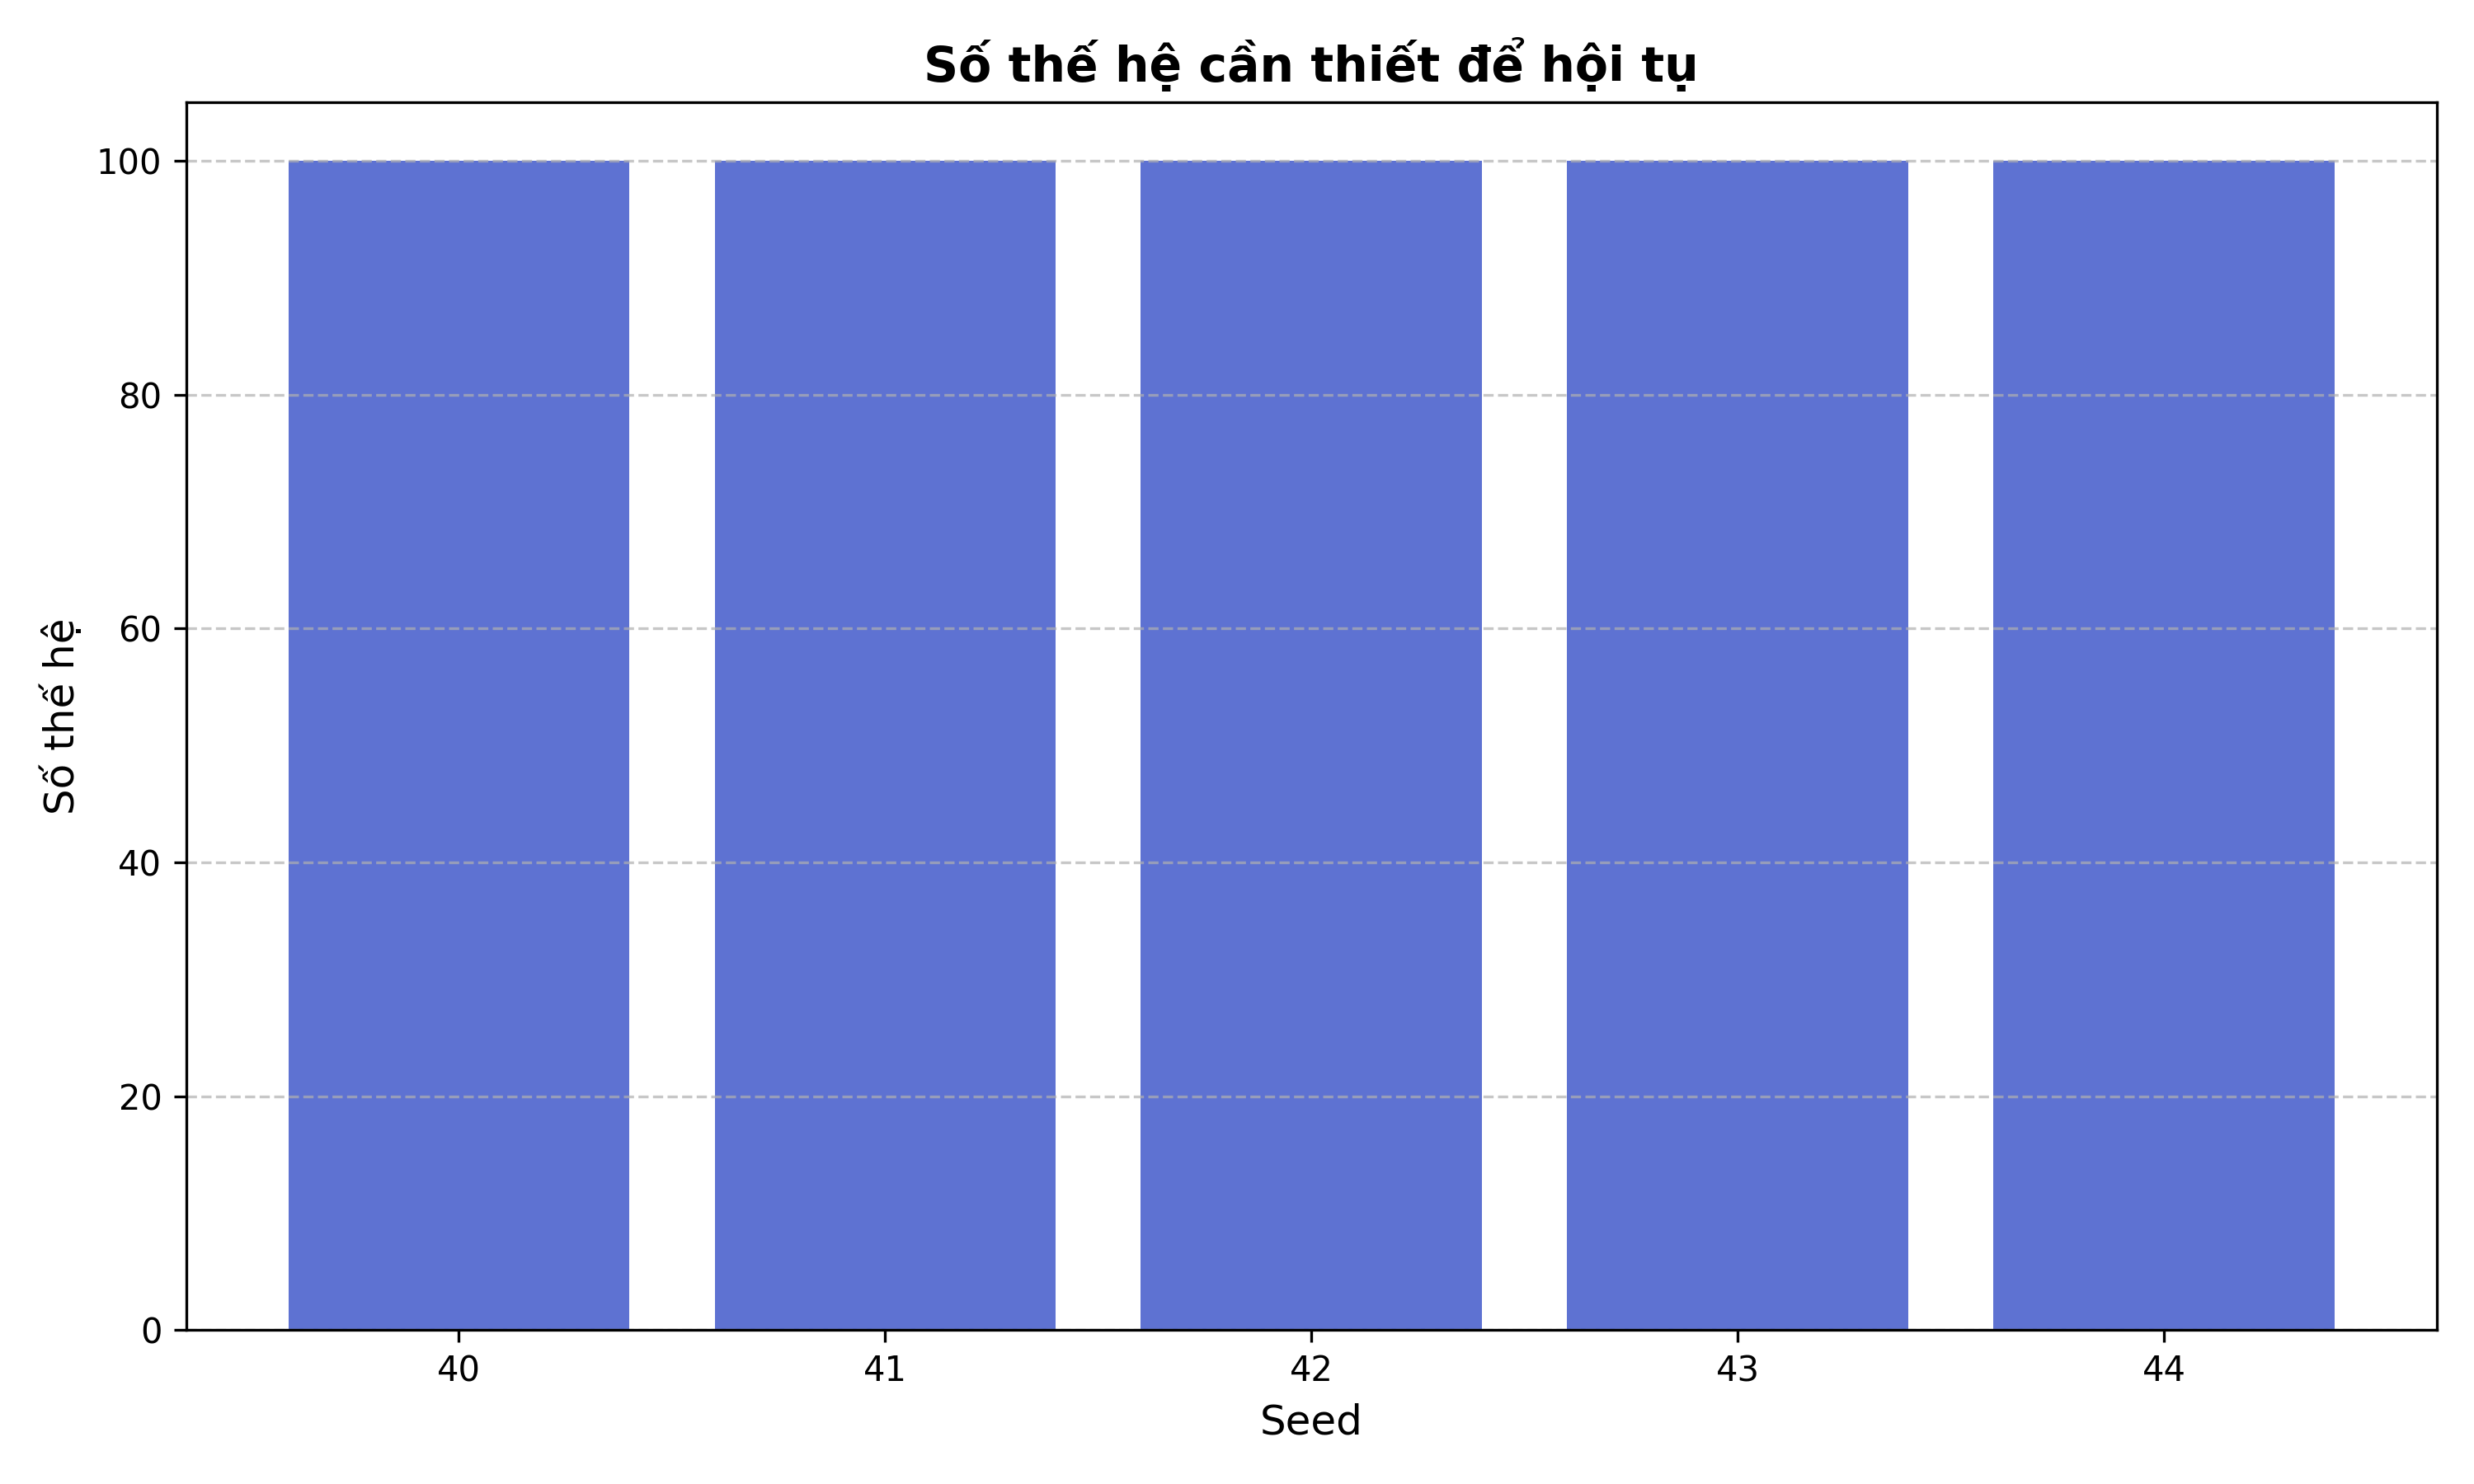
\includegraphics[width=\textwidth]{images/convergence_speed.png}
        \caption{Tốc độ hội tụ của thuật toán qua các lần chạy.}
    \end{minipage}
    \caption{Phân tích tương quan giữa chất lượng nghiệm và tốc độ thực thi của hệ thống.}
    \label{fig:comparison}
\end{figure}
